\documentclass[../main.tex]{subfiles}

\begin{document}

\chapter{Background} \label{chapter:background}

This chapter describes the relevant theory behind software bug predictions and what the state of the art has been able to achieve. 

\section{Machine Learning} 

Machine learning can be defined as the study of algorithms that learn from a set of observed samples to predict values for unseen samples \cite{koza1996automated}. These algorithms have recently gained traction and become more applied in products and services due to the increase in computing power, availability of open source machine learning frameworks and vast amounts of data. Machine learning has become a popular approach for software defect prediction models as they eliminate the need for a programmer to explicitly set rules that identify a commit or file as being risky or not. Machine learning approaches can automatically spot patterns in data that may have been difficult for people to find, especially if the dimensionality of the input space is large. Some of the main challenges with these algorithms are to obtain substantial quantities of data and to ensure that the model's predictions are reliable.

In the context of software defect prediction, machine learning models are used to solve a binary classification problem. Classification involves taking samples of data and identifying their correct category (\textit{risky} or \textit{not risky}) given their features. There are various algorithms available for classification which differ by their mathematical formulations.

\subsection{Logistic Regression}

Logistic regression is a binary classification model that takes real valued inputs and returns their probability of belonging to one of two classes, 0 or 1. The logistic regression model makes predictions by applying the sigmoid function $\sigma(z) = \frac{1}{1+e^{-z}}$ upon a linear model $f(x) = x^T\theta$ (where $x$ is our input and $\theta$ is the model's parameters) \cite{bishop2006pattern}. When provided an input vector $x$, the function $\sigma(f(x))$ will predict the probability that $x$ belongs to the class 1 whereas $1-\sigma(f(x))$ computes the probability the class of $x$ is 0. The final label that is predicted is based on the most likely class, for example if the output of $\sigma(f(x)) > 0.5$, the predicted class is 1.  

The optimal parameter for $\theta$ can be found using maximum likelihood estimation which aims to find the parameter $\theta$ that maximizes the likelihood $p(\textbf{t}|\theta)$ (where $\textbf{t}$ a vector containing output labels). Typically, this maximization problem is transformed into a minimization problem by taking the negative log of the likelihood. Then, iterative methods such as gradient descent can be used to obtain the optimal parameters. 


\subsection{Decision Trees}

Decision trees are a type of tree-based model which classify inputs by using a set of conditional rules \cite{grzymala1993selected}. Every node in the decision tree represents a single conditional rule applied to an input feature, for example a dataset containing information about people could be split into two subsets by using the rule $Age < 30$. After a decision rule has been evaluated, the input is passed further down the tree along one of two possible branches. One heuristic algorithm used for creating a decision tree is ID3 which constructs a tree using a greedy, top-down approach \cite{quinlan1986induction}. Given a dataset $D$ and some features, ID3 chooses a feature that has not been included in the tree yet such that it provides the largest information gain. A decision rule is created upon this feature and this allows a dataset to be partitioned. The algorithm stops when all features are used up or when all elements of a partition have the same label. 
 
\subsection{Ensemble Methods}

An issue with decision trees is that an individual tree can be very prone to overfitting the training data, resulting in a high variance model. In order to combat this, one can rely on ensemble techniques which involve combining multiple base models when training. One example of an ensemble learning technique is bagging which trains multiple classifiers independently and aggregates their outputs \cite{breiman1996bagging}. Given that we want to train $n$ models, bagging will randomly sample the training set and train a model on this sample so that each individual model has a different view of the data. A random forest model applies bagging by training $B$ decision trees. When a prediction has to be made for a classification task it aggregates the predictions by taking the majority value from each tree. 

Boosting methods on the other hand involve sequential training of an ensemble of classifiers to convert weak classifiers (a model that does slightly better than random) into stronger ones \cite{sewell2008ensemble}. Unlike in bagging methods such as random forest, the classifiers are dependently trained on each other. When trained sequentially, subsequent models will attempt to correct upon previous learners by giving an increased weight to data points that the last model misclassified. Some examples of commonly used boosting methods applied upon decision trees are AdaBoost and XGBoost. 

\subsection{K-Nearest Neighbours}

The K-nearest neighbours algorithm is another example of a non-parametric algorithm. To make a prediction for a new data point $x$, the algorithm must find the $k$ elements of the training set that are closest to $x$ \cite{cunningham2007k}. The proximity of points can be measured using distance metrics such as Euclidean distance or similarity metrics like the Pearson correlation \cite{jaskowiak2011comparing}. The predicted label for $x$ will then be the most frequent label among its k-nearest neighbours. In the case of a binary classification problem, $k$ should be chosen to be odd to guarantee that a majority label exists. When the labels of the dataset are imbalanced (such as in the case of defect prediction models), the algorithm might predict the dominant class more due to how frequently it occurs rather than because it is the correct label \cite{coomans1982alternative}. In this case, one can apply a weighted aggregation of the $k$ labels so that closer data points contribute more to the final prediction.  


\subsection{Semi-Supervised Learning}

The majority of software defect prediction models are done using supervised learning where models are provided labelled datasets that they can learn from and make predictions for new data. Semi-supervised learning on the other hand relies on labelled and unlabelled data to train models. The motivation for semi-supervised approaches is that labelling data can be expensive, therefore, the idea is to use unlabelled data as much as possible together with limited labelled data. 

According to \cite{chapelle2006semi}, in order for semi-supervised learning to be effective, there are several assumptions that have to be made. First of all, data points that are close to each other or form clusters should have a high probability of having the same label. This is because semi-supervised methods propagate labels from labelled instances to unlabelled instances. Also, it is required that points in higher dimensions need to be representable in lower dimensions in order for points to be able to considered close to each other. 

\subsection{The Self-Training Algorithm} \label{section:selfTrain}

The self-training algorithm is a type of semi-supervised algorithm that can act as a wrapper method for any classifier \cite{triguero2015self}. When provided labelled and unlabelled data, the algorithm begins by training a classifier on the labelled data. It then makes predictions for the unlabelled data and if the classifier's prediction has a high probability, these predicted samples will be included in the training dataset. Then a model trains on this new dataset and these steps are repeated until the maximum number of iterations are reached or if the predictions for unlabelled data is identical to the previous iteration's predictions. 

For the self-training algorithm, let us define the following. Let $X_L, y_L$ be our labelled inputs and outputs. $X_U$ is the unlabelled dataset and the model is defined as the function $f:X \rightarrow Y$. The parameters for the algorithm are $I \in \mathbb{N}$, the max number of iterations and $C \in \{c \in \mathbb{R} | 0 \leq c \leq 1\}$, the minimum confidence for a prediction on unlabelled data. The vairable $iter$ represents the current iteration and $y_{U\_old}$ is a local variable for storing the previous predictions. The variable $idx$ contains the indices of all unlabelled samples such that their probability of being either class is greater than the threshold $C$. 

Some variations of this algorithm will move samples from $X_U$ and their predicted labels to the sets $X_L,y_L$. This version on the other hand samples does not remove entries from the unlabelled dataset.

\begin{algorithm} [H]
    \caption{Self-training algorithm \cite{zhu2007semi}}
    \label{algorithm:selfTrain}
    \begin{algorithmic}[H]
        \Procedure{Self-Train($X_{L}, y_{L}, X_{U}, I, C, ',f$)}{}
            \State $iter = 0$
            \State $f = f.fit(X_L, y_L)$
            \State $y_U = f.predict(X_U)$
            \State $y_{U\_old} =$ an empty array with same length as $y_U$
            
            \While{iter $<$ I and $|y_{U\_old}| == 0$ or $y_U \neq y_{U\_old}$}
                \State $y_{U\_old} = y_{U}$
                
                \State $idx = \{1 \leq i \leq len(y_U) | P(y_i=1) > C$  $\vee$ $P(y_i=0) > C\}$
                
                \State $X_{new} = \{x_i \in X_U | i \in idx\}$  
                \State $y_{new} = \{y_i \in y_U | i \in idx\}$
                
                \State $f = f.fit(X_L.concat(X_{new}), y_L.concat(y_{new})$

                \State $y_U = f.predict(X_U)$

                \State iter = iter + 1

            \EndWhile
            \State return $f$
        \EndProcedure
    \end{algorithmic}
\end{algorithm}



One variation of this algorithm involves using no thresholds when adding the unlabelled data to the labelled data. One can also make predictions on a smaller batch of unlabelled rather than on all possible unlabeled data. As the algorithm works as a wrapper method to any base classifier, it is possible to make a direct comparison between a supervised learning algorithm and its self-trained counterpart. A risk with using this algorithm is that its performance could degraded if it spots an incorrect pattern early on and reinforces this on the unlabelled data. 

\section{Evaluating Classification Models}

In order to verify that our models have performed well at a classification task, the models are evaluated on a test set and various performance measures are recorded. Below are metrics that describe the possible outcomes that can occur when making a prediction:

\begin{itemize}
    \item $TP=$ The number of true positives, instances belonging to the target class that were correctly identified
    
    \item $TN=$ The number of true negatives, instances belonging to the non-target class that were correctly identified
    
    \item $FP=$ The number of false positives, instances belonging to the non-target class that were misclassified as the target class
    
    \item $FN=$ The number of false negatives, instances belonging to the target class that were misclassified as the non-target class
\end{itemize}

In the context of software defect prediction, a false positive (FP) would describe a commit that was actually clean but predicted to be risky. A false negative (FN) would be a commit that was risky but classified as not risky. These four values can be used to reason about a model's performance and define further performance metrics. 

\subsection{Accuracy, Precision, Recall and F1 score}

\vspace{20pt}

\begin{equation}
    Accuracy = \frac{TP+TN}{TP+TN+FP+FN}
\end{equation}

\vspace{10pt}

Accuracy represents the fraction of total data samples our model predicted correctly. However, if a dataset has a class imbalance (which software defect prediction datasets typically do), accuracy can be a misleading metric for performance. Since one of the classes would be underrepresented, the machine learning classifiers learn to simply predict the majority class label for every sample it sees. Take the following example, with a dataset of emails where 99\% are not spam and 1\% are spam, a classifier could achieve 99\% accuracy by labelling each email as not containing spam. However, this would lead to a very high number of false negatives and the classifier would not have actually learned what a spam email is. Therefore we rely on additional metrics such as precision and recall.

\begin{equation}
    Precision = \frac{TP}{TP+FP}
\end{equation}

\begin{equation}
    Recall = \frac{TP}{TP+FN}
\end{equation}

\vspace{20pt}

Precision in the context of software defect prediction is the fraction of instances that were correctly classified as defective relative to all instances that were deemed defective by the classifier. Recall is the fraction of correctly identified defects relative to the actual number of defective instances. Precision and recall are inversely proportional to each other, therefore as soon as a classifier aims to optimize recall, its precision will decrease and vice-versa. 

\begin{equation}
    F1 = 2*\frac{precision*recall}{precision+recall}
\end{equation}

The F1 score aims to combine precision and recall into one metric using the harmonic mean so that one can optimize models towards having a good combination of both.

\begin{comment}
\subsection{Receiver Operating Characteristic Curves}

The Receiver Operating Characteristic (ROC) curve is an indication of how well the model can tell apart various classes at various thresholds. By default, a classifier such as logistic regression sets its threshold at 0.5, if the output is greater than 0.5 then we assign an instance to one class and if it is lower than 0.5 it gets assigned to the other class. However, one can vary this threshold in order to deal with situations where the cost behind a false negative is not equally weighted with the cost of a false positive (for example, letting a bug go unnoticed versus a developer spending time reviewing supposedly faulty code that is actually clean). 

\begin{figure}[H]
\centering
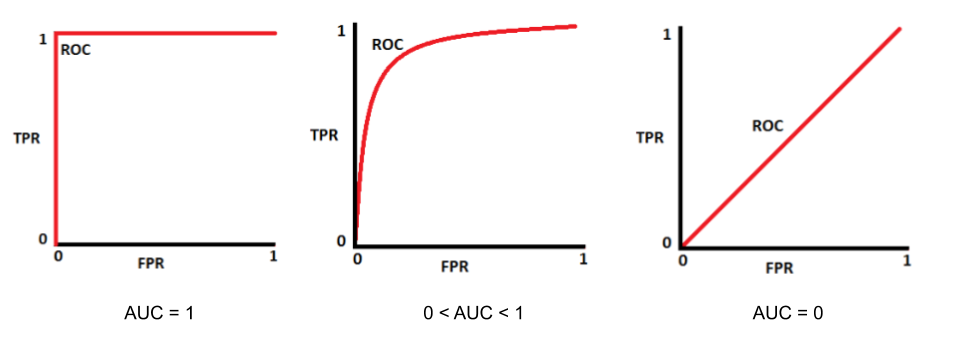
\includegraphics[scale=0.45]{images/Background/roc_cases.png}
\label{fig:roc}
\caption{The possible cases for the ROC-AUC \cite{rocCases}}
\end{figure}

The ROC curve plots the false positive rate (FPR) and the true positive rate (TPR), also referred to as the recall. To quantify the performance of the classifier for various thresholds, the Area Under Curve (AUC) metric is used. As seen in figure \ref{fig:roc}, ideal classifiers have $AUC = 1$ because their true positive rate is 1 regardless of the false positive rate. In the worst case, the $AUC = 0.5$ and this indicates that model cannot distinguish between the two classes. When the $AUC$ is less than 0.5, this indicates that the model is able to distinguish between the two classes but the labels are swapped.

\subsection{Precision-Recall Curves}

According to Davis \cite{davis2006relationship}, an issue with ROC curves is that they are insensitive to class imbalance. Because of this, a high ROC-AUC value can be misleading when measuring the performance of software defect prediction models. Davis suggests that one should also rely on precision-recall curves which plot the precision and recall of a classifier for various thresholds. Similar to ROC curves, one can compute the AUC of these curves to get an aggregate measure of how well the model performs. 

\end{comment}

\subsection{K-fold Cross Validation}

K-fold cross validation is a statistical method for generalizing a model's performance to unseen data \cite{kale2011cross}. Cross validation has two main roles, the first being for model selection during training and the second is for evaluating a model's final performance. K-fold cross validation involves splitting up a dataset into $k$ partitions such that a classifier trains on $k-1$ of the partitions and is evaluated on the remaining set (designated the test set). When performing model selection, a dataset will typically be split into a training, validation and test set. The validation set is used to tune the hyperparameters of a model whereas the test set is used for a final evaluation.

A benefit of using cross validation is that it reduces bias and error when estimating the classifier's true performance. However, there is criticism for using cross validation as an evaluation method for software defect predictions. This is because a model may end up using future knowledge by training on samples that occurred later in time than those in the test set \cite{tan2015online}. 

\subsection{Metrics for Semi-Supervised Classifiers}

When evaluating the semi-supervised classifier, one can measure how well the model's predictions are for unlabelled data it used during training. One can define the reconstruction accuracy as the fraction of unlabelled instances from the training set that the self-training algorithm provided correct predictions for. Since the self-training algorithm runs for several iterations, this reconstruction accuracy is computed once the algorithm has terminated. Also, each iteration the algorithm can technically make a prediction for the same instance if the prediction never meets the confidence threshold, thus never being transferred from the unlabelled training set to the labelled training set. Therefore the predictions that will be considered in the reconstruction error are those that were added to the labelled training set. Similarly, one can define the reconstruction precision and reconstruction recall in order to investigate if there are discrepancies between the correctness of labels for the two classes.

\section{Related Work}

This section outlines some of the past achievements in the field of software defect prediction and the various techniques that were used. 

\subsection{Software Defect Prediction}

The purpose of software defect prediction is to predict the likelihood of a defect within software. The proposed benefit of these models would be to assist software developers with bug detection and to prioritize testing efforts \cite{briski2008minimizing}. The general process for constructing software defect prediction models begins with obtaining a dataset that labels files or commits as \emph{risky} or \emph{not risky} (a risky commit is defined as a commit that will produce a bug). Then for each instance in the dataset (a commit or file), various features such as McCabe complexity or lines of code are computed \cite{zhang2007predicting}. The features and labels are then used to train a supervised machine learning classifier and finally, the model can be used to make predictions for new instances. 

When building defect prediction models, there are various input features one could use. one could provide metadata concerning files or commits such as lines of code added or the number of developers working on a particular file. One could also use text based features such as commit messages or comments which can be encoded using a bag-of-words representation. One could also parse the source code itself with abstract syntax trees which can be encoded as vectors \cite{tan2015online}.

%TODO \subsubsection{File Level Defect Prediction}

\subsection{SZZ Algorithm}

In order to build defect prediction models, one requires labelled data that indicates whether or not a file or commit contains a bug or not. However in practice, this information may not always be available and manually labelling commits is time consuming. Research in defect prediction models have benefited greatly from the Sliwerski Zimmermann Zeller (SZZ) algorithm, originally described in the paper \textit{"When do changes induce fixes?"} \cite{sliwerski2005changes}. The focus of the paper was limited to identifying bug inducing commits rather than creating defect prediction models but their labelling algorithm is valuable for automatically labelling a large number of commits. 


\begin{algorithm}
\caption{SZZ: labels commits as \textit{risky} or \textit{not risky} \cite{sliwerski2005changes}}
\label{algorithm:szz}
    \begin{algorithmic}[1]
    \Procedure{SZZ()}{}
        \State $\texttt{keywords}=\{"bug","fix"\}$
        \State \texttt{commits} = a list of all commits in a repository
        \State \texttt{bugFixCommits} = $\{\texttt{c :c} \in \texttt{commits}\texttt{ and }\texttt{containsKeyword(c.message)}\}$ 
        \State \texttt{result =} $\emptyset$
        \For{\texttt{i = 1 to length(bugFixCommits)}}
                \State \texttt{bugFixCommit = bugFixCommits[i]}
                \State \texttt{filesTouched = getFilesTouched(bugFixCommit)}
                \State \texttt{linesTouched = getLinesTouched(bugFixCommit, filesTouched)}
                \State \texttt{result = result $\cup$ getBlame(filesTouched, linesTouched)}
        \EndFor
    
        \State \texttt{return result}
    \EndProcedure
    \end{algorithmic}
\end{algorithm}

The algorithm works by initially locating commits that fix a bug. This can be done by filtering commits by their message or comments for keywords such as "bug" or "fix". Those commits are then cross referenced with a bug tracking database in order to confirm that these commits do resolve a bug. For each bug fixing commit, the files this commit touched as well as the exact lines changed within those files are computed using the \texttt{diff} command in a version control system (such as CVS or Git). One can then use the \texttt{blame} or \texttt{annotate} command to find the previous commit responsible for causing a patch to be created. This previous commit becomes labeled as a bug causing commit. A variant of this algorithm denoted Approximate SZZ follows the same essential steps but does not rely on a bug tracking database for identifying bug fixing commits. Since not all projects use a bug tracking database, using the ASZZ algorithm would allow defect prediction models to train on more data. 

%SZZ revisited: verifying when changes induce fixes, Jaime Spacco (2008)) Claims that no one has previously verified the reliability of the SZZ algorithm. Outlines several improvements to SZZ, replace annotation graphs with line number maps, use DiffJ to ignore comments and formattinf changes in soure. Then finally verify that SZZ identified the correct changes. Manually select 25 bug fixing commits random commits from 37,000 commits of the Eclipse projects. These 25 commits changed 50 lines in total. Only 43 of the 50 changed lines actually fix a bug. (They evaluate reliability of finding bug-fix commits). 

\subsection{File Level Defect Prediction }

In their work, Meng Yan et al. investigate the claim that unsupervised models may outperform supervised models for providing effort-aware defect predictions on the file level \cite{yan2017file}. They replicate a previous study upon the PROMISE dataset and their main finding was that unsupervised models can outperform supervised models for cross project prediction but not for within project predictions. 

In Personalized Defect Prediction, the authors propose creating defect prediction models that are tailored to individual developers \cite{jiang2013personalized}. The motivation for this is the fact that developers exhibit varying coding patterns and styles and the number of bugs introduced can depend upon the experience the developer has. Results found that this method can improve a model's F1 score by 0.01-0.06.

Song Wang et al. apply a Deep Belief Network upon the file-level changes of software projects \cite{wang2016automatically}. Their deep learning models are trained upon vector representations of the programs' Abstract Syntax Trees and this approach was shown to improve within-project as well as cross-project defect prediction. The issue with non-semantic metrics (such as lines of code) is that programs performing different tasks may have the same values for these metrics. Their models were evaluated upon 10 open source Java projects from the PROMISE datasets. Their evaluation compares to two baselines, the first being non-semantic features that were available in the PROMISE datasets and the second being AST nodes that they provided to their models. 


\subsection{Just-in-time Defect Prediction}

A method for providing software defect predictions that has gained traction recently is Just-in-time defect predictions. These models make predictions at the commit level rather than at the file level and utilize commit metadata for features rather than product metrics or by analyzing the source code \cite{kamei2013large}. The motivation for this approach is the fact that commits tend to be smaller and more manageable to review than files. Also, there is the fact that files can be edited by multiple developers which makes it challenging to assign an individual developer to resolve the bug whereas commits only have one author \cite{kamei2013large}. A proposed benefit of these models is having the ability to provide immediate feedback to a developer as soon as a change is made. 

One of the earlier works on change-level defect prediction, \textit{"Classifying Software Changes: Clean or Buggy?"} suggested that one should train models on file changes rather than files or functions themselves \cite{kim2008classifying}. This paper differs from previous work in the sense that it used the SZZ algorithm to find the exact changes that cause a bug whereas previous work relied on bug-fix data which could only show roughly where a bug occurred. Also, due to the fact that they represent their features using a bag-of-words encoding, their technique could work independently of programming language. 

In their paper, Kamei et al. \cite{kamei2013large} introduce the idea of Just-in-time prediction models where models attempt to predict risky commits rather than risky files. They also ensure that the bug-fixing commits that the SZZ finds are present in a bug-tracking database for each project they investigate. They evaluated their models on six open source projects as well as five commercial projects to obtain an average accuracy of 68\% and average recall of 64\%. They also evaluate if the model serves a useful purpose practically, i.e. will prioritizing commits by risk level reduce the amount of work required when reviewing code. This paper is considered to be the most related to the research undertaken within this thesis as the same datasets and similar modelling techniques are used. 

A follow up work to the previous paper stated that predictions have to be feasible for projects that have little historical data available \cite{fukushima2014empirical}. This can be a challenge for defect prediction models where the model only trains on data from a single repository. Instead, they investigate the feasibility of cross project models, models that train on data from multiple projects. They find that within-project models do not perform well on cross-project performance. They also found that within project models can improve if the project they intend to predict on has similar correlations between predictor and dependent variables. It was shown that file level predictions seem to do better at cross project performance than commit level predictions. Finally, they also show that ensemble learning techniques benefit cross project performance. 

In "Deep learning for just-in-time defect prediction", the authors propose a deep-learning based approach to detect risky commits \cite{yang2015deep}. They evaluate performance on the same 6 OSS projects that Kamei et al. used and showed that their approach outperformed previous models. They use a deep belief network algorithm for feature selection and then utilized deep neural networks to build the classifier. Their model named Deeper was able to find 39.96 \% more bugs and had statistically significant higher F1 scores. This paper was one of the first examples of applying deep learning to this field and they also investigate the effect that the quantity of data has on their model.

Yang et al. try a different approach to Just-In-Time (JIT) predictions that involves a 2-layer ensemble learning classifier named TLEL that combines stacking and bagging techniques with decision trees \cite{yang2017tlel}. The first layer consists of applying bagging to a decision tree to produce a random forest model. The second layer uses stacking and random undersampling to train multiple random forest models and combine them together. The motivation behind this two-layer approach according to them is that they observed that decision tree perform particularly well at this task as well as the fact that ensemble methods tend to produce better results over single models. They compare their approach to three previous models, Deeper, DNC and MKEL. For evaluating their models, they rely on F1 score and PofB20 which measures the cost effectiveness of the model (how well the model can find bugs by only reviewing 20\% of all lines of code). 

In the paper "Supervised vs Unsupervised Models: A Holistic Look at Effort-Aware Just-in-Time Defect Prediction", they limit their focus on effort aware JIT defect prediction which tries to find risky commits while inspecting the code as minimally as possible \cite{huang2017supervised}. They state that one challenge in this field is obtaining labelled training data so they investigate the possibility of using unsupervised models. Their contribution is the CBS algorithm CBS (Classify Before Sorting) which makes predictions and then sorts the output by the size of the commit in ascending order. They focus on making their predictions effort aware because it takes time to inspect a commit and they want to minimize the time a developer would need to do a review after they receive predictions. They also observed that the distribution of lines of codes in commits is skewed, the majority of commits are small and very few are large, thus the need for applying logarithmic transformations to their features.

In his paper "Online Defect Prediction for Imbalanced Data", Ming Tan addresses the challenge of class imbalance in defect prediction \cite{tan2015online}. Usually, the minority of entries in datasets will have a label corresponding to a bug. The author tried out four resampling methods which alter the training set in order to deal with the imbalance in the dataset. Another issue that is brought up is that previous studies rely on cross validation to evaluate model performance which does not assess models in a realistic manner. The reason being that cross validation splits up the training and test sets in a way such that models can use future knowledge to make predictions. Instead, the author suggests that a time-sensitive classification should be used so that the test set only contains commits that occur later in time than the commits provided in the training set. 

\subsection{Practical Implementations of JIT Prediction Models}

A recent open source implementation of a JIT risk prediction model would be Commit Guru which builds directly on top of the work presented in "A large-scale empirical study of just-in-time quality assurance" \cite{rosen2015commit}. Commit Guru is able to take a GitHub repository and returns statistics on which commits may have high risk. The associated paper outlines the architecture of the tool as well as the usage of the SZZ algorithm and the classification model they use. As \cite{nayrolles2018clever} points out, the limitation of this tool is that it cannot point out which exact code block caused a bug. Also, there has not been a formal study that investigates how useful the predictions are for developers and what performance we should expect in terms of precision and recall for developers to trust the tool. 

The video games developer Ubisoft performed a study in collaboration with Concordia University in which they developed a tool named CLEVER which builds upon Commit Guru when performing predictions of risky commits \cite{nayrolles2018clever}. They rely on a two stage process, the first is similar to Commit Guru as it predicts commits that are risky. The second step then does a deeper analysis of those potentially risky commits by comparing code snippets with a database of known bugs to confirm that the commit does cause some sort of issue and is not a false positive. 

\end{document}





\begin{comment}
\subsection{Challenges in defect prediction}

\subsubsection{Imbalanced data}

TODO

Due to the fact that the majority of changes to a codebase will function as intended, there will be an imbalance in the dataset between the two classes of risky and not risky. Machine learning algorithms tend to see a drop in performance when trained on imbalanced data.. For example, given a classifier tasked with diagnosing cancer in patients where the rate of having cancer is 5\%, the algorithm would be accurate 95\% of the time if it simply diagnosed every patient as not having cancer. Despite the high accuracy, this would be a very poor classifier in practice as it hasn't actually learned to spot the minority class. The classifier performs this way because the risky samples are underrepresented so it assumes that in most cases, a label would not be risky. There is also the fact that false positives and false negatives are by default weighted equally but in practice a false negative tends to be worse than a false positive. In our example of defect prediction, it is much worse if a bug is introduced and goes unnoticed as opposed to having a developer inspect some code and find no bugs. 


https://medium.com/james-blogs/handling-imbalanced-data-in-classification-problems-7de598c1059f

Typical approaches to address this involve re-sampling methods such as over sampling and undersampling. These methods increse or decrease instances of a class in a dataset until there is a 50/50 split. 
\subsubsection{Skew in data}
\subsubsection{Collinearality between features}
\subsubsection{Within project vs cross project models}

Within projects models are defined to be models trained on a single repository whereas cross project models learn from a mix of previous projects. The importance of making this distinction is because defect prediction models should be able to make predictions on new projects with little historical data available. However, machine learning models in practice require a large amount of data to perform well. 
%http://posl.ait.kyushu-u.ac.jp/~kamei/publications/Fukushima_MSR2014.pdf

Their report found that having a high within-project performance can still lead to a low cross project performance. Kamei et al found that 

\end{comment}
